% 本手法が実用に適することと性能限界を示す ... 埋め込みのreliabilityを評価した
% reliabilityとは、現実的な状況で埋め込まれたwatermarkが十分に解読できることの保証である
To verify proposed watermarking method to be feasible and to show the performance limit of that, we evaluated the reliability of watermark embedding, guarantee that watermarks embedded in practical situations can be detected correctly with adequate certainty.
% 様々な設定で透かしの収録を行い、デコード可能なwatermarkの割合(CDR)を測定した
We recorded videos embedding watermarks with various watermarking settings, and measured the correct detection rates (CDRs) of watermarks in each.
% 実際の映像撮影は様々な場面で行われ、環境音の現れも多様であるため、以下の実験はsilent/public/rock/electronicという4つの音響条件下でそれぞれ行い、いずれの状況でもreliabilityが確保されるかを試した
Generally, videos are recorded in diverse situations; therefore characteristics of environmental sound also vary depending on them.
Taking it into consideration, we conducted following experiments in four different environmental settings, those are silent room, public space, playing rock music and playing electronic music, to see that embedding reliability of our method is retained in any situations.

% まず、どの程度の量のデータを安定に埋め込めるかを評価するため、bit rateを色々変化させてCDRを測定した。
% bit rateはdata frameが短いほど高くなるので、data frame長を6ms(666bps)から10ms(400bps)まで1ms刻みで変化させて5種類の実験を行った
% 各watermarkはランダムな16bytesのデータで、3秒おきに100個のwatermarkを連続で埋め込んでデコードした
Firstly, we measured CDRs changing the data rate of watermarking to evaluate how much data can be embedded per unit time stably.
Since the length of a data frame decides the data rate of watermarking, we changed it from 6 ms to 10 ms at 1 ms intervals.
6 ms length of a data frame corresponds to about 666 bps data rate, and 10 ms corresponds to 400 bps.
For each data frame lengths and environmental settings, one hundred watermarks with 16 bytes payloads were embedded at 3 seconds intervals, and the correctly detected watermarks were counted using our watermark decoder after recordings.
Figure \ref{fig:eval_reli_btrt} shows the measured CDRs in each condition.
This result shows that enough reliability can be gained in any recording environments if the data frame length is set 10 ms.
CDRs dropped rapidly as data frame length decreased below 10 ms, especially in the environment with electronic music.
It is probably due to the high-frequency tones contained in the music that confuse watermark detector.
From the result, we concluded that 10 ms was the optimal value for the length of a data frame.

% bit rate依存のreliability変化
\begin{figure}[htbp]
 \begin{center}
  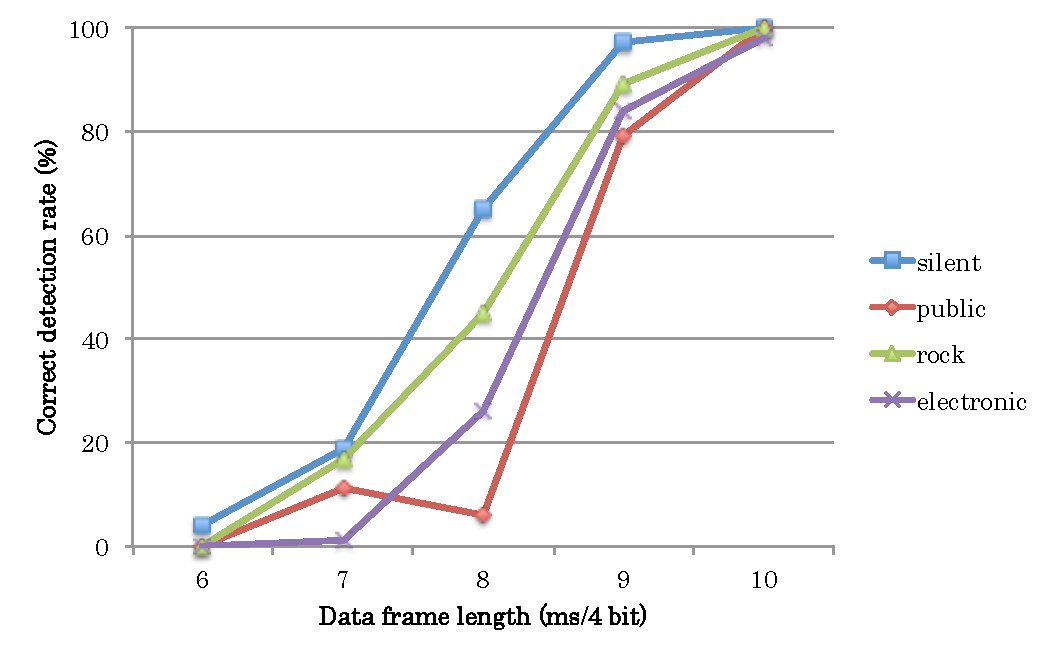
\includegraphics[width=120mm]{evaluation_reliability_bitrate.pdf}
 \end{center}
 \caption{The correct detection rates (CDRs) at variable data rates.}
 \label{fig:eval_reli_btrt}
\end{figure}
% 結果は〜

% 次に、安定に埋め込めるパケットの大きさを評価するため、payload長を色々変化させたpacketを埋め込んでCDRを測定した。
Secondly, we conducted a similar experiment changing the payload length of a packet to confirm that even a large data can be embedded as a watermark stably.
% 8, 16, 32, 64, 128 bytes の5条件
In this experiment, one hundred watermarks with a certain payload length from 8 bytes to 128 bytes were recorded in a video, and the CDR was measured later.
% data frame lengthは10msに固定
The data frame length of watermarks was fixed 10 ms.
% 結果
The result shown in Figure \ref{fig:eval_reli_pyld} demonstrates that CDR was slightly decreased with payload length increasing, but retained above 95\% at all payload lengths and situations.
% 色々なタイプのデータを格納するのに利用することが出来る
This means that our method can be used to embed many kinds of annotations with various data sizes, from an integer value to a long string like a caption sentence.

% payload依存のreliability変化
\begin{figure}[htbp]
 \begin{center}
  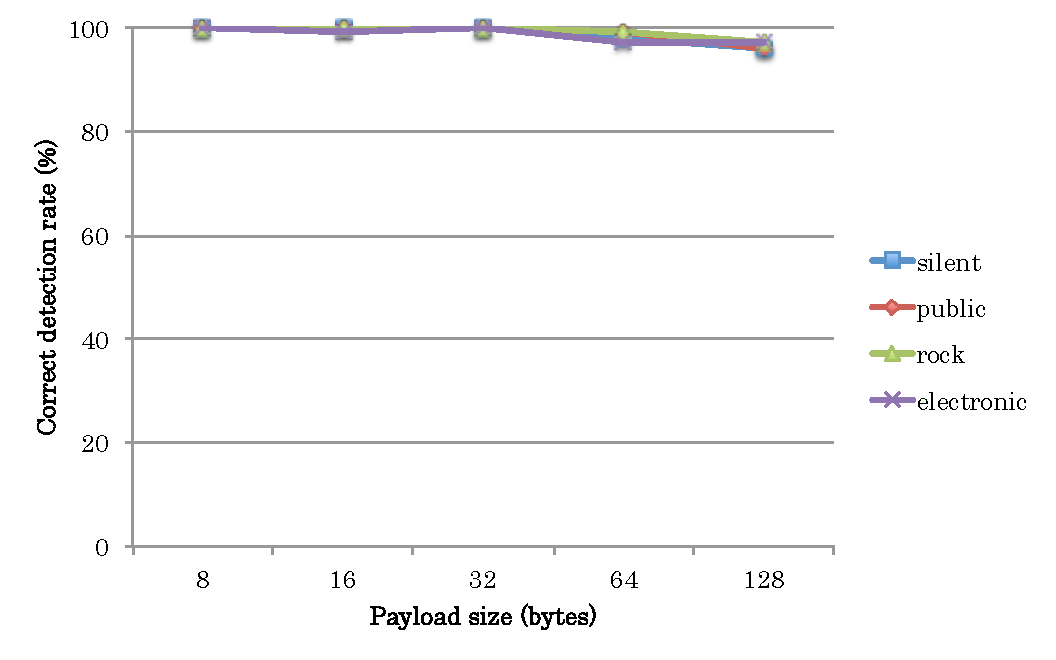
\includegraphics[width=120mm]{evaluation_reliability_payload.pdf}
 \end{center}
 \caption{The correct detection rates (CDRs) at variable payload sizes.}
 \label{fig:eval_reli_pyld}
\end{figure}

% しかし100%ではないので、何らかの冗長化機構をプロトコルに組み込むことを考えても良いかもしれない
However 100\% CDR is not guaranteed always in principle, these two experiments showed that AnnoTone's watermarking technique has adequate reliability for various usage in diverse recording situations.
If more accurate CDR was needed in any usage, we could append an error correction mechanism to our watermarking scheme at the expense of data rate.
